\documentclass[a4paper,12pt]{article}
\usepackage{graphicx}       %LaTeX package to import graphics

\usepackage[T1]{fontenc}
\usepackage[italian]{babel}

\usepackage{subcaption}

\usepackage{hyphenat}
\usepackage{array}
\usepackage{booktabs}       % Per linee orizzontali migliori
\usepackage{caption}        % Per personalizzare le didascalie<
\usepackage{multirow}       % Per combinare celle nelle colonne
\usepackage{float}
\usepackage{hyperref}

\usepackage{bm} 

\usepackage{amsmath}        % Per migliorare l'aspetto delle formule

\usepackage{todonotes}      % mettere le note dentro il documento

\usepackage{siunitx}        % Per formattare le unità di misura
\usepackage{gensymb}        % Simboli come °
\usepackage{xfrac}          % per fare le frazioni inclinate

\usepackage{pdfpages}

\usepackage{import}
\usepackage{frontespizio}

\usepackage{placeins}       %per non far andare le immagini al di fuori delle sezioni utilizzare il comando: \FloatBarrier non far superare le immagini quel punto

\usepackage{adjustbox}      % per dimensionare le immagini in modo automatico


\begin{document}

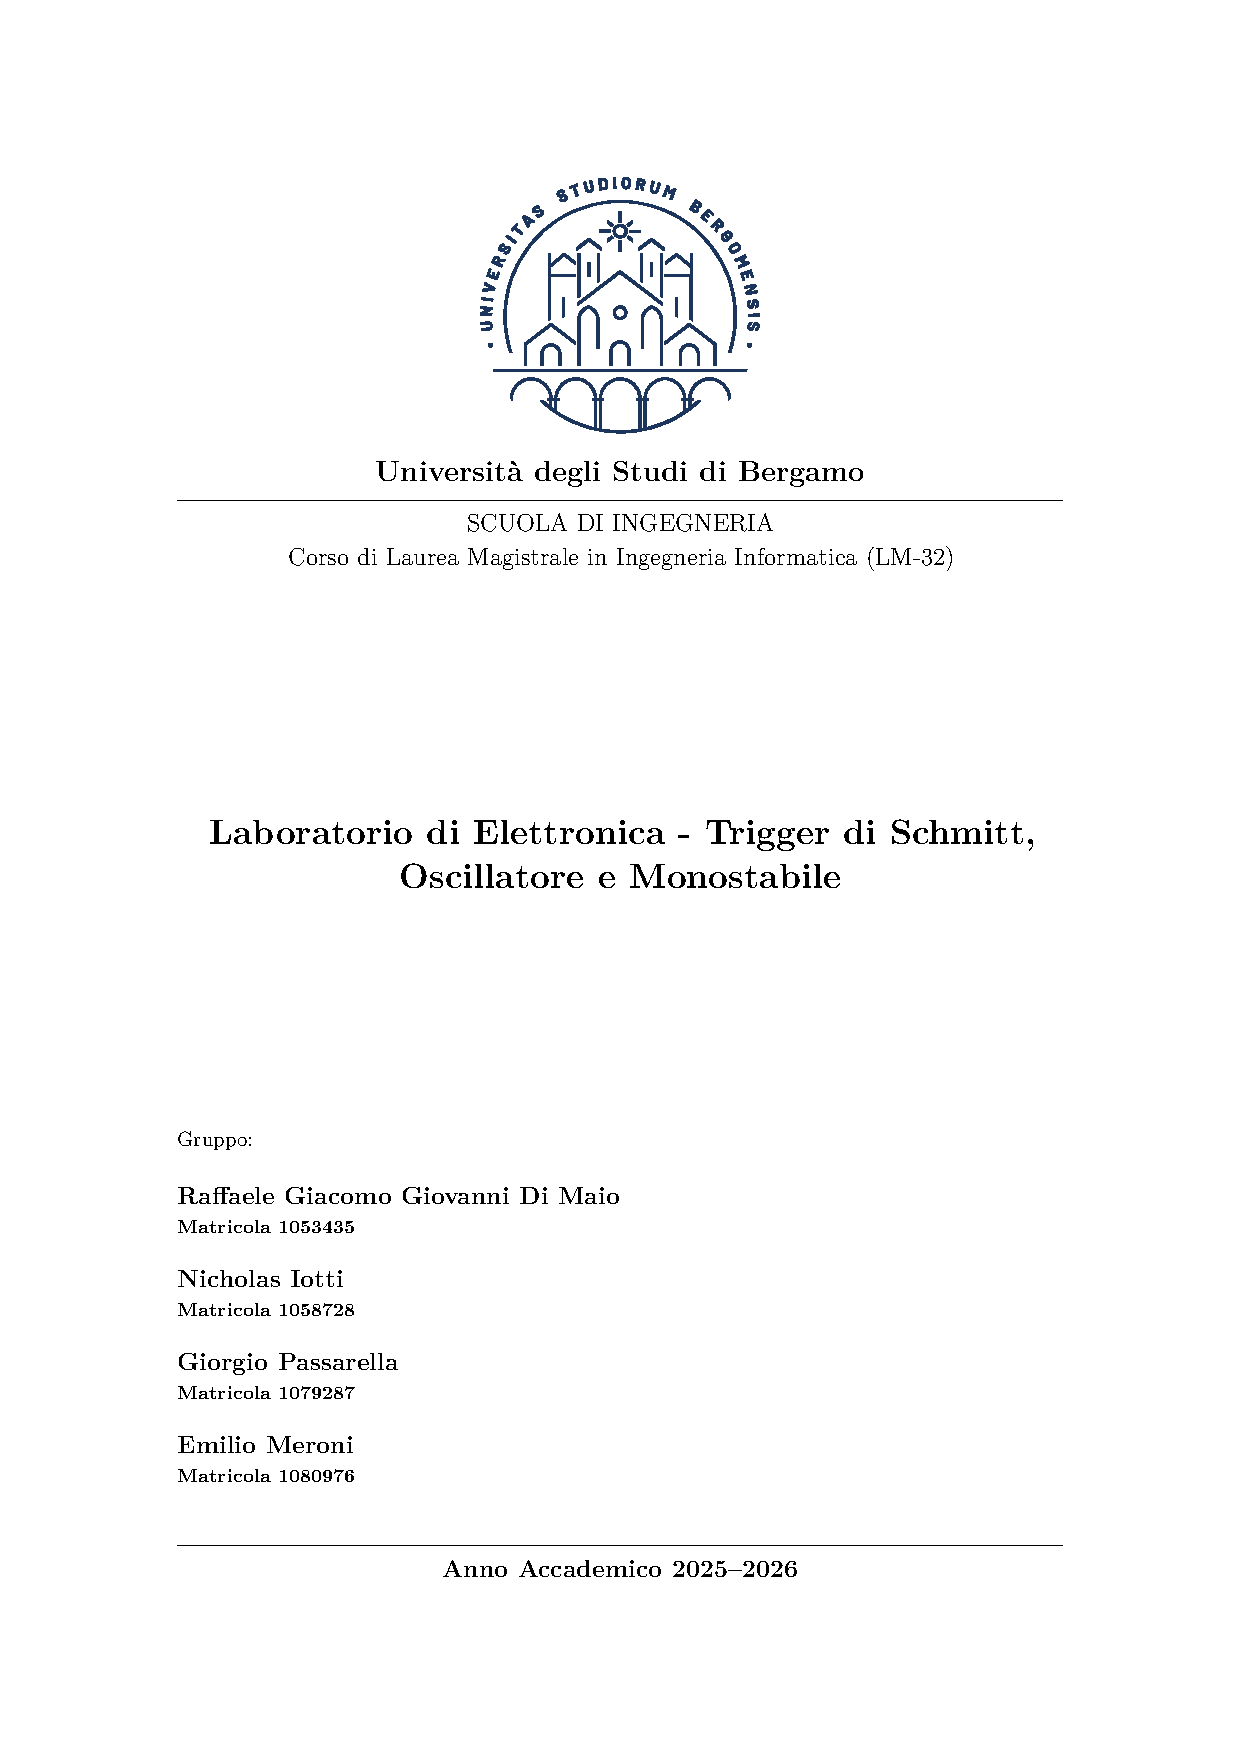
\includepdf{./frontespizio/frontespizio.pdf}

\section*{Trigger di Schmitt}
L'amplificatore operazionale è un circuito elettronico che permette di confrontare due tensioni in ingresso e fornirne la differenza tra le due moltiplicata per un fattore di amplificazione $A$.
\begin{align*}
	V_{out} = A \cdot (V^+ - V^-)
\end{align*}
Nel caso ideale $ A \rightarrow \infty $, pertanto l'uscita $V_{out}$ saturerà alla tensione di alimentazione positiva $V_{DD}$ solo se la differenza tra le due tensioni è maggiore di zero, altrimenti $V_{out} = -V_{DD}$.
Questo permette di utilizzarlo come comparatore di due tensioni. Tuttavia nella realtà sono presenti delle problematiche dovute alla presenza di rumore elettronico che porta il segnale in uscita ad avere degli scatti spuri dovuti al ripetuto passaggio della soglia a causa del rumore stesso.
Per risolvere questo problema si utilizza il trigger di Schmitt, figura \ref{fig:trigger_schmitt}.

\begin{figure}[h]
	\centering
	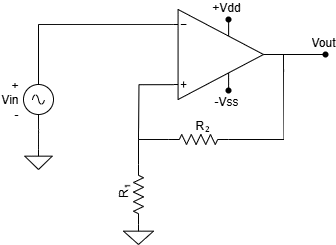
\includegraphics[width = 0.55\linewidth]{./immagini/schmitt/circuito.png}
	\caption{Schematico del Trigger di Schmitt}
	\label{fig:trigger_schmitt}
\end{figure}

Grazie all'utilizzo di una soglia dinamica, dipendente da $V_{out}$, permette di avere in uscita un segnale meno sensibile al rumore in ingresso. In particolare la soglia si modifica secondo questi punti:
\begin{enumerate}
	\item Ipotizzando uno stato iniziale in cui $V_{in} \ll 0$ allora si ha che $V_{out}$ satura a $V_{DD}$, questo porta ad avere un potenziale in $V^+$ pari a:
	      \begin{align*}
		      V^+ = \frac{R_1}{R_2 + R_1} \cdot V_{DD} \xrightarrow{\mathrm{Hp:}\,R_1 = R_2} \frac{V_{DD}}{2} = V^+_H
	      \end{align*}
	      determinando la soglia;
	\item Quando $V_{in} > V^+_H$ allora $V_{out}$ diventa pari a $V_{SS}$, ciò comporta ad avere $V^+ = \frac{V_{SS}}{2} = V^+_L$, ovvero una nuova soglia;
	\item Infine, si rimane nello stato $2$ fino a quando $V_{in}$ diventa inferiore di $V^+_L$, se si supera la soglia si riparte dal punto $1$.
\end{enumerate}
Questo andamento genera un ciclo di isteresi con ampiezza pari a:
\begin{align*}
	A =\frac{2R_1}{R1+R2} \cdot V_{DD} \xrightarrow{\mathrm{Hp:}\,R_1 = R_2} V_{DD}
\end{align*}
La quale si può verificare a figura \ref{fig:schmitt_mod_xy}.

\begin{figure}[h]
	\centering
	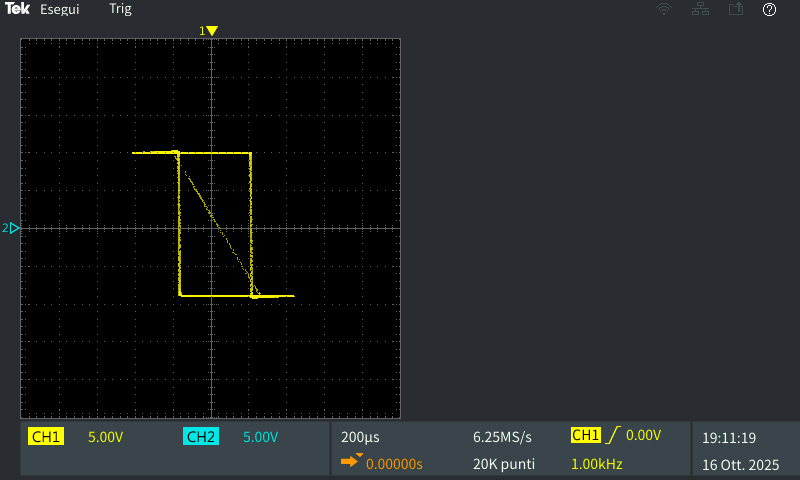
\includegraphics[width = 0.8\linewidth]{immagini/schmitt/schmitt_vin_vout_xy.png}
	\caption{Ciclo di isteresi del Trigger di Schmitt, con ampiezza di circa $10\,\mathrm{V}$}
	\label{fig:schmitt_mod_xy}
\end{figure}

\noindent I valori utilizzati per testarne il funzionamento sono riportati a tabella \ref{tab:valori_trigger_schmitt}:
\begin{table}[h]
	\centering
	\setlength{\tabcolsep}{20pt}
	\begin{tabular}{c c}
		\toprule
		\textbf{Grandezza}     & \textbf{Valore}            \\
		\midrule
		$V_{DD}$     & $10\,\mathrm{V}$  \\
		$V_{in\,pp}$ & $20\,\mathrm{V}$  \\
		$freq$       & $1\,\mathrm{KHz}$ \\
		$R_1$        & $9.0\,K\Omega$    \\
		$R_2$        & $9.0\,K\Omega$    \\
		\bottomrule
	\end{tabular}
	\caption{Valori utilizzati nel circuitio: Trigger di Schmitt.}
	\label{tab:valori_trigger_schmitt}
\end{table}

\noindent I grafici ricavati sono riportati a figura \ref{fig:schmitt_oscilloscopio}.


\begin{figure}[h]
	\centering
	\begin{subfigure}{0.49\linewidth}
		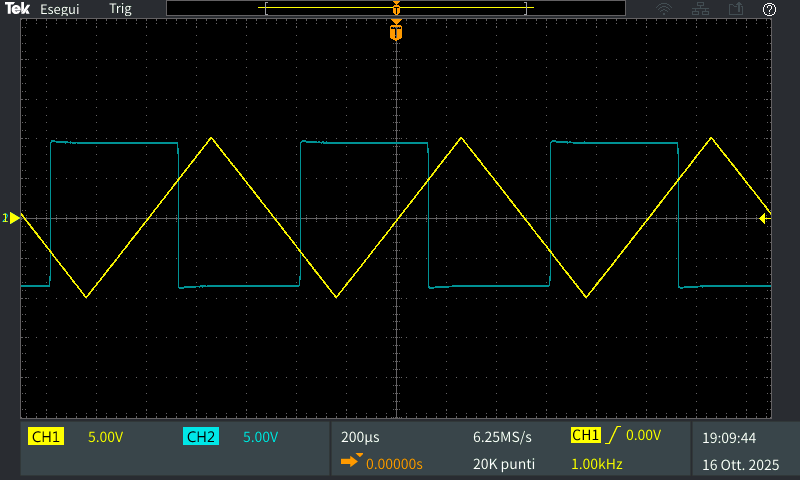
\includegraphics[width = \linewidth]{immagini/schmitt/schmitt_vin_vout.png}
		\caption{}
	\end{subfigure}
	\begin{subfigure}{0.49\linewidth}
		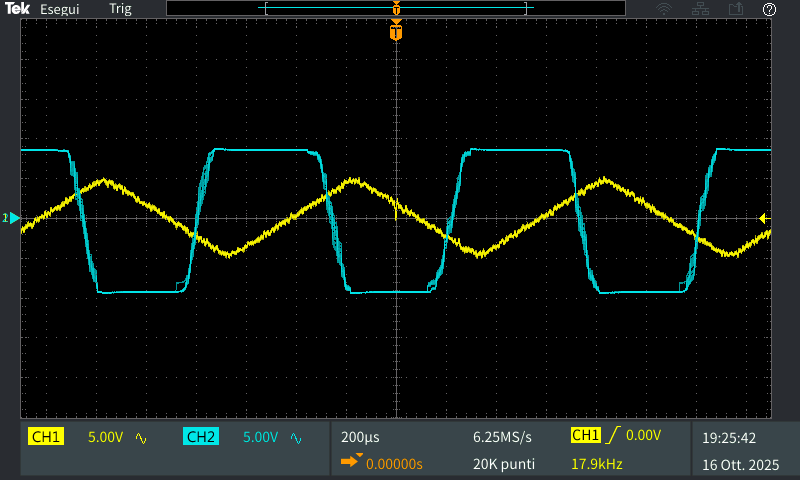
\includegraphics[width = \linewidth]{immagini/schmitt/schmitt_vin_vout_rumoroso.png}
		\caption{}
	\end{subfigure}
	\\[0.5cm]
	\begin{subfigure}{0.49\linewidth}
		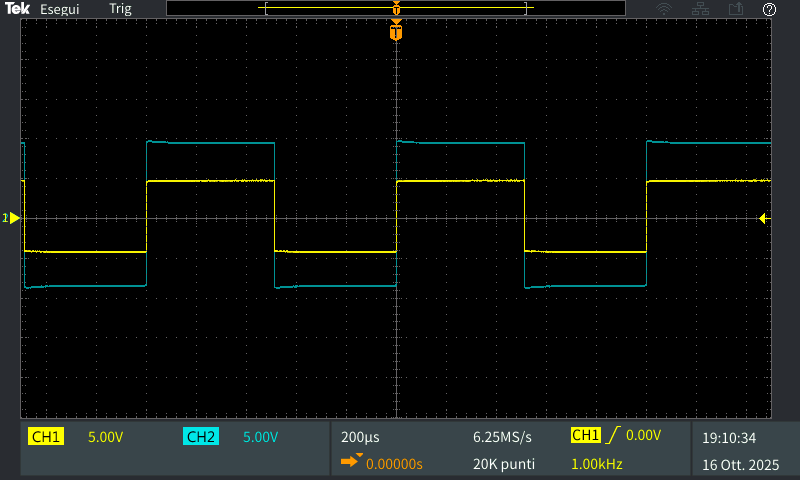
\includegraphics[width = \linewidth]{immagini/schmitt/schmitt_v+_vout.png}
		\caption{}
	\end{subfigure}
	\begin{subfigure}{0.49\linewidth}
		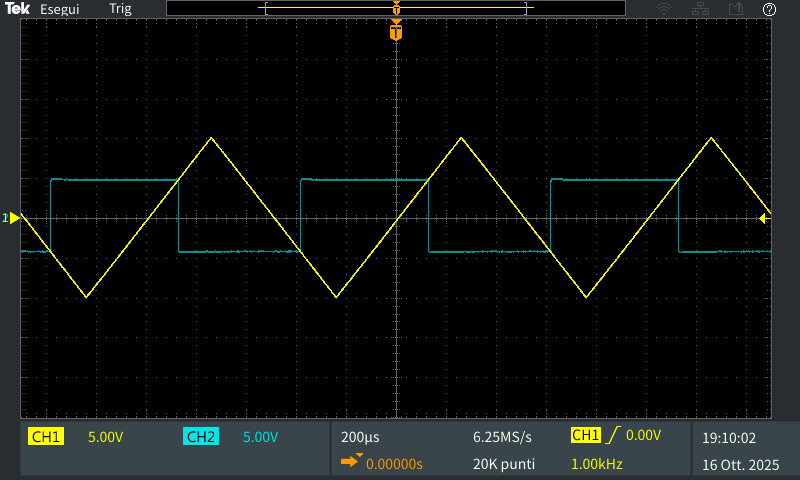
\includegraphics[width = \linewidth]{immagini/schmitt/schmitt_vin_v+.png}
		\caption{}
	\end{subfigure}
	\caption{Figure \textit{a} e \textit{b}: $V_{in}$ in giallo e $V_{out}$ in azzurro, confronto con segnale in ingresso non rumoroso (\textit{a}) e rumoroso (\textit{b}).
		Figura \textit{c}: in giallo la soglia dinamica, $V^+$, in azzurro l'uscita.
		Figura \textit{d}: Soglia dinamica confrontata con l'ingresso (in giallo).}
	\label{fig:schmitt_oscilloscopio}
\end{figure}

\FloatBarrier

\section*{Oscillatore}
L'oscillatore è un circuito elettronico che genera un segnale ad onda quadra, in questa particolare implementazione si sfrutta il \textit{Trigger di Schmitt} e la carica/scarica di un condensatore, figura \ref{fig:schematico_oscillatore}.
\begin{figure}
	\centering
	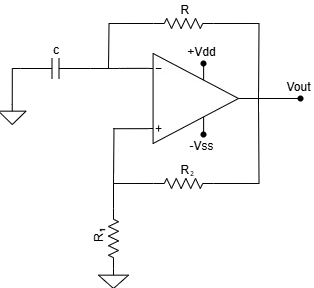
\includegraphics[width=0.5\linewidth]{immagini/oscillatore/circuito.png}
	\caption{Schematico oscillatore.}
	\label{fig:schematico_oscillatore}
\end{figure}
Il funzionamento del circuito si può suddividere in due fasi:
\begin{itemize}
	\item $V_{out} = V_{DD}$: La corrente fluisce da destra verso sinistra caricando il condensatore con una costante di tempo $\tau = R \cdot C$; inoltre il potenziale nel morsetto positivo dell'amplificatore è pari a:
	      \begin{align*}
		      V^+ = V^+_H \xrightarrow{\mathrm{Hp:}\,R_1 = R_2} \frac{V_{DD}}{2}
	      \end{align*}
	      Si rimane in questa condizione finché la capacità non si carica fino ad avere una caduta di tensione pari (o maggiore) a $V^+_H$.
	\item Nel momento in cui $V^-$ supera $V^+$ in uscita si ottiene $V_{SS}$, la quale modifica la $V^+$ portandola a una tensione pari a $V^+_L = \frac{V_{SS}}{2}$. In questa condizione la corrente in $R$ scorre da sinistra verso destra, scaricando il condensatore fino a quando la tensione in $V^-$ diventa inferiore a $V^+_L$ portando di nuovo il circuito nello stato precedente.
\end{itemize}
Tramite l'equazioni di carica e scarica:
\begin{align*}
	V_c (t) = V^- (t) & = V_{\text{finale}} + (V_{\text{iniziale}} - V_{\text{finale}} ) \cdot e^{-\sfrac{t}{\tau}}
\end{align*}
Si può determinare i tempi un cui $V_{out}$ è alta e bassa, determinando così il valore della frequenza di oscillazione.
\begin{align*}
	\text{Carica}\,\,  & \Rightarrow V_{DD} + (V^+_L - V_{DD}) \cdot e^{-\sfrac{T_1}{\tau}} = V^+_H \\
	\text{Scarica}\,\, & \Rightarrow V_{SS} + (V^+_H - V_{SS}) \cdot e^{-\sfrac{T_2}{\tau}} = V^+_L
\end{align*}
Per le quali utilizzando $\left| V_{DD} \right| = \left| V_{SS} \right|$ si ottiene:
\begin{align*}
	T_1 = T_2 = \tau \ln\left( \frac{R_2 + 2R_1}{R_2} \right) \xrightarrow{R_1 = R_2} \tau \ln \left( 3 \right)
\end{align*}
Questo risultato ci porta concludere che il duty cylce è pari al $50\%$, e la frequenza di oscillazione è pari a $ f = \frac{1}{T_1 + T_2}$, la quale e inversamente proporzionale alla costante di tempo $\tau$.

\noindent I valori utilizzati questo circuito sono indicati a tabella \ref{tab:oscillatore}, a figura \ref{fig:oscillatore} viene mostrato l'andamento dell'uscita al variare di $V^-$. Infine si sono effettuate diverse prove per confermare la relazione $f \propto \sfrac{1}{\tau}$ modificando la resistenza variabile $R$, figura \ref{fig:oscillatore_freq_tau}.

\noindent Mantenendo $\left| V_{DD} \right| = \left| V_{SS} \right|$, l'oscillatore avrà sempre un duty cycle pari al $50\%$, se si volesse modificarlo si potrebbero utilizzare due resistenze diverse, una per la carica e una per la scarica, utilizzando due diodi per far scorrere la corrente nel modo corretto.
\begin{table}[h]
	\centering
	\setlength{\tabcolsep}{20pt}
	\begin{tabular}{c c}
		\toprule
		\textbf{Grandezza} & \textbf{Valore}               \\
		\midrule
		$V_{DD}$ & $10\,V$              \\
		$R_1$    & $9.0\,K\Omega$       \\
		$R_2$    & $9.0\,K\Omega$       \\
		$R$      & Resistenza variabile \\
		$C$      & $70\,\mathrm{nF}$    \\
		\bottomrule
	\end{tabular}
	\caption{Valori utilizzati nell'oscillatore.}
	\label{tab:oscillatore}
\end{table}

\begin{figure}[h]
	\centering
	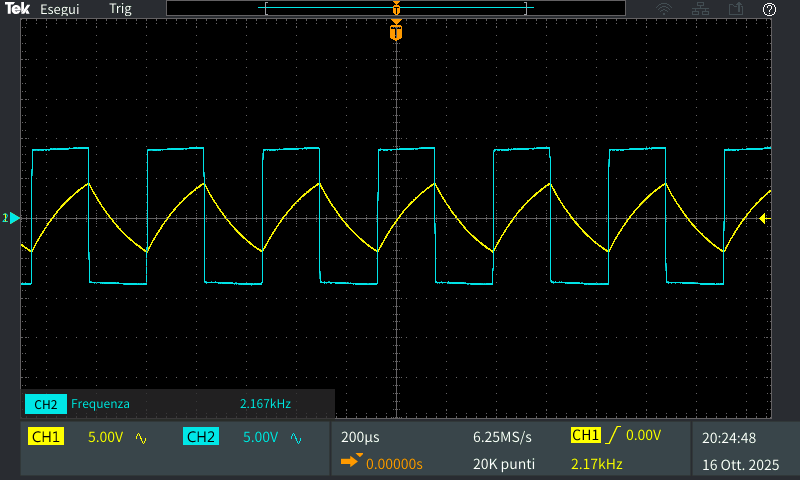
\includegraphics[width=0.7\linewidth]{immagini/oscillatore/oscillatore.PNG}
	\caption{Schermata dell'oscilloscopio, in giallo $V^-$ mentre in azzurro l'uscita $V_{out}$.}
	\label{fig:oscillatore}
\end{figure}

\begin{figure}[h]
	\centering
	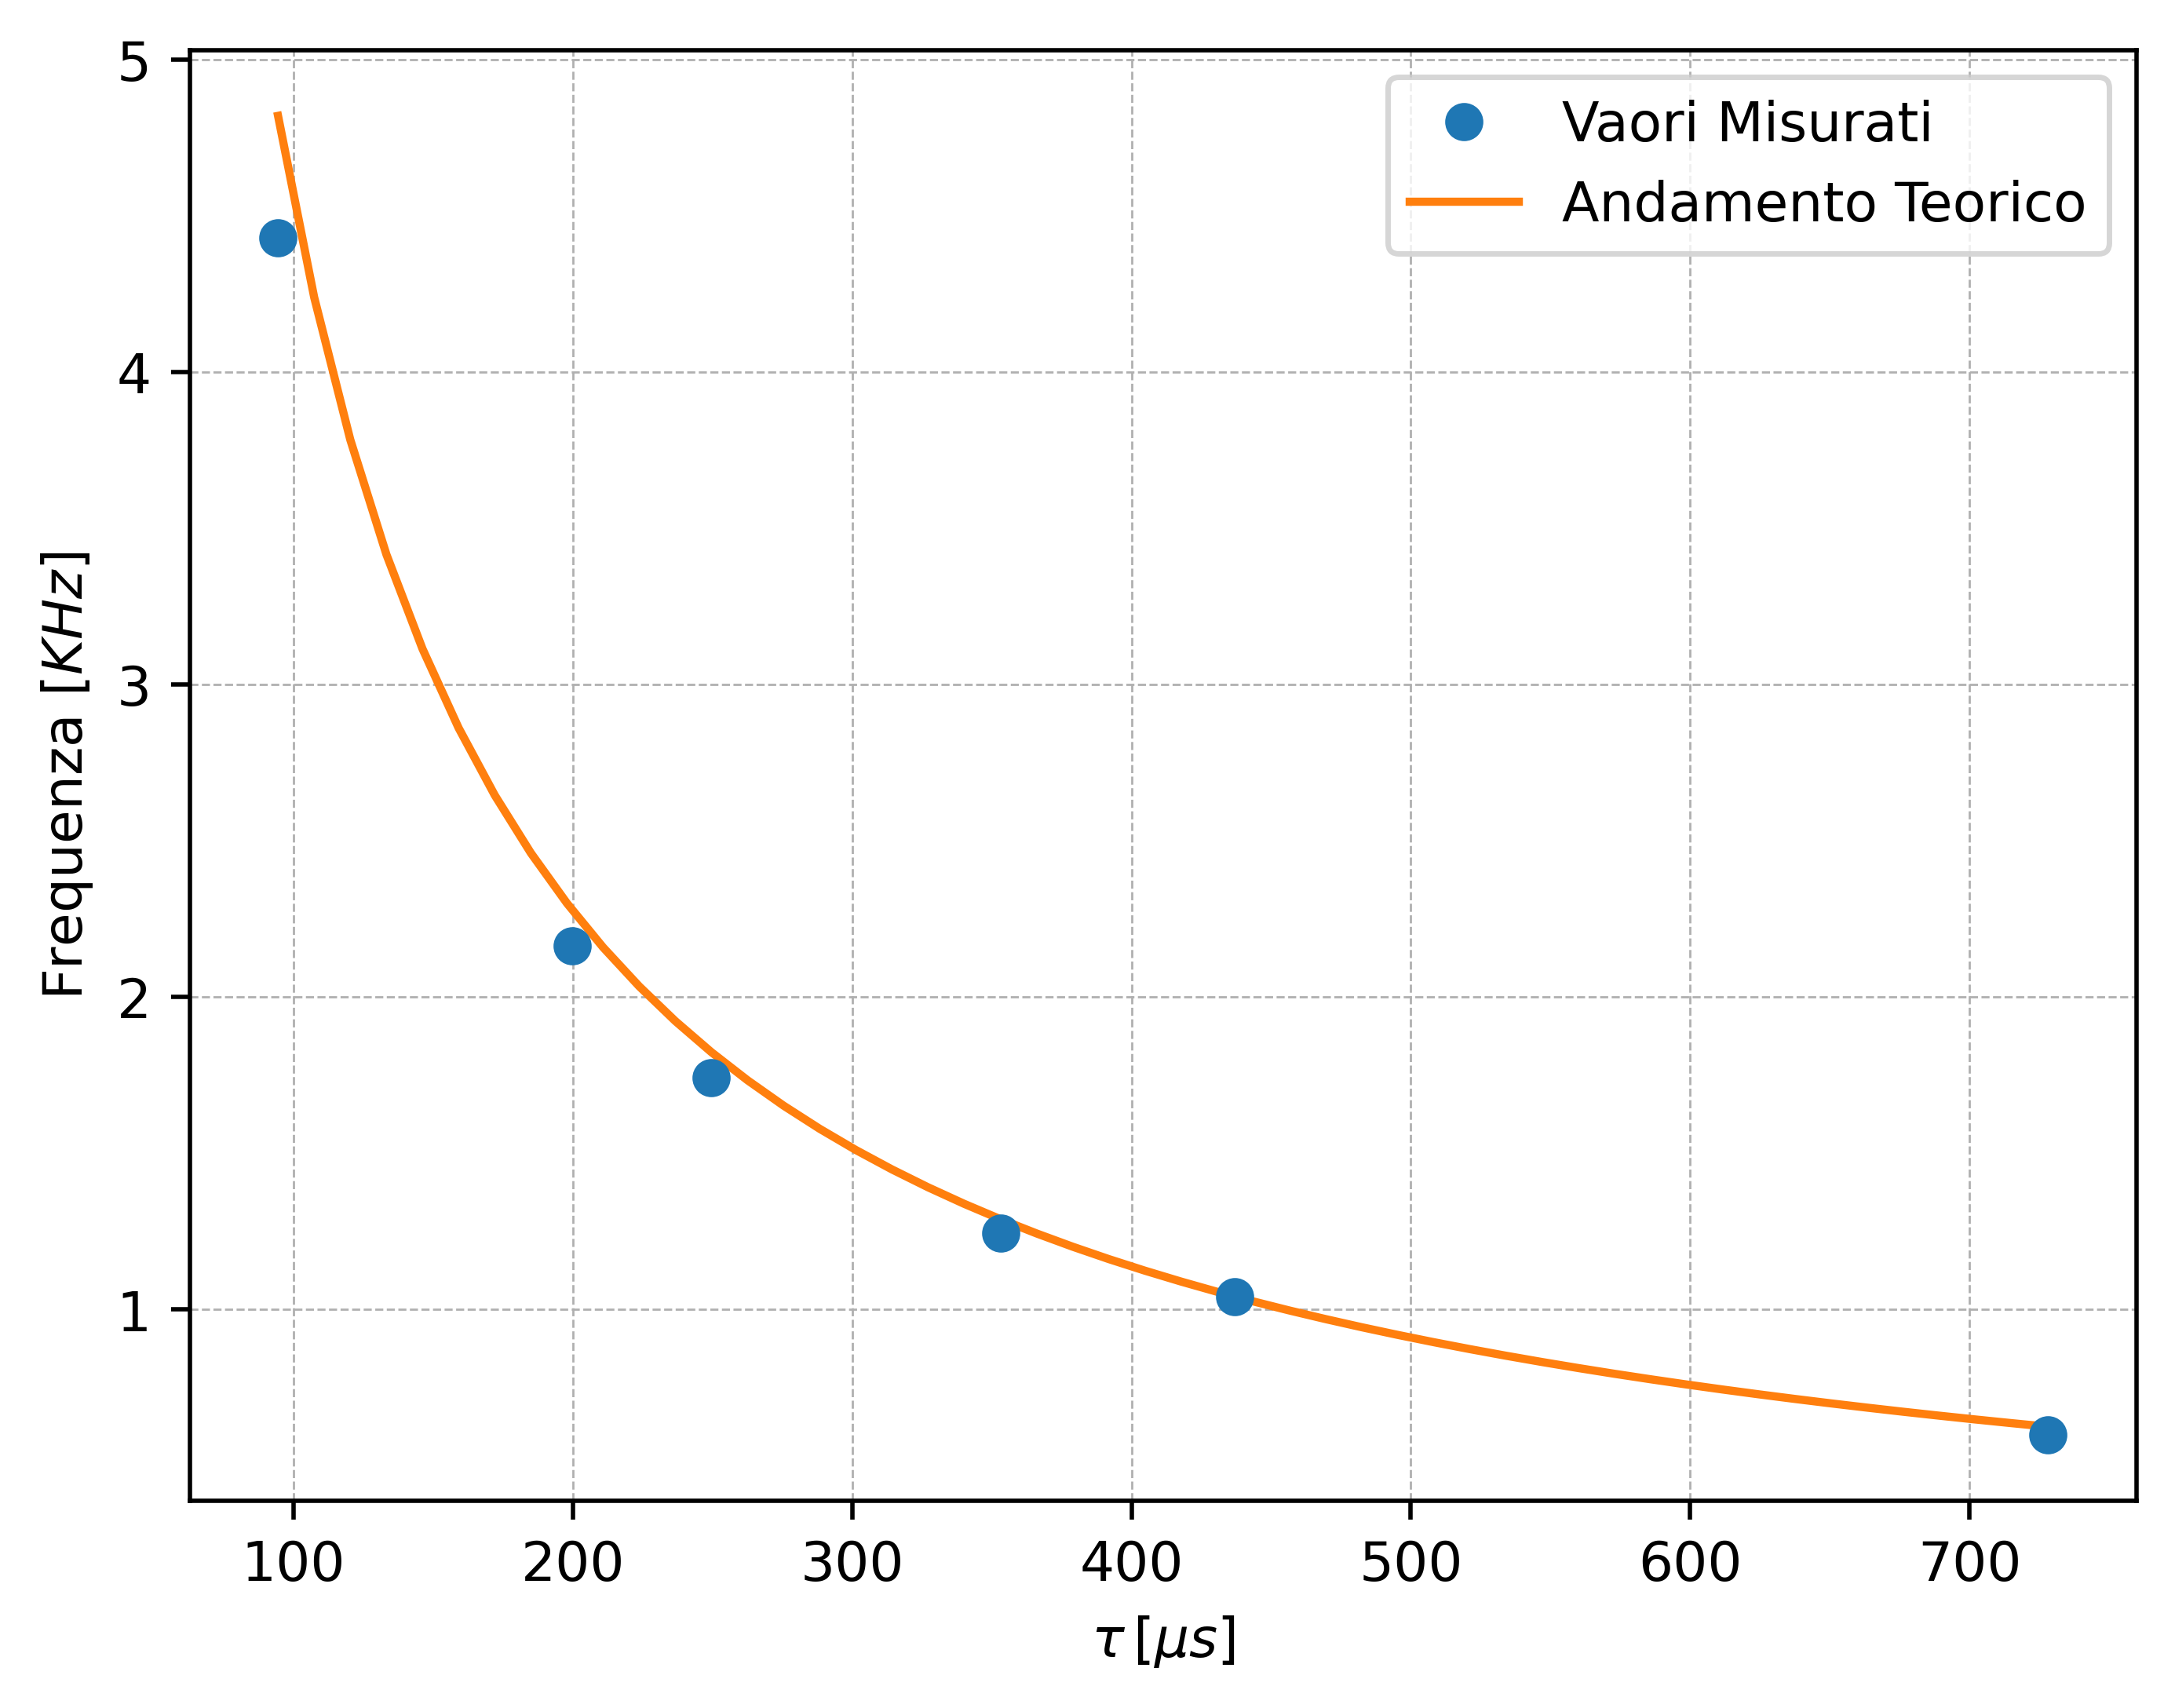
\includegraphics[width=0.6\linewidth]{immagini/oscillatore/freq_tau.png}
	\caption{Variazione della frequenza al variare della costante di tempo $\tau$.}
	\label{fig:oscillatore_freq_tau}
\end{figure}
\FloatBarrier

\section*{Monostabile}
Il Monostabile è un circuito elettronico che riceve in ingresso un segnale e dà in uscita un impulso di durata ben definita.
Inoltre, il fronte d'onda ascendente del segnale in uscita è sincronizzato con il fronte d'onda discendente del segnale in ingresso.

\begin{figure}[h]
	\centering
	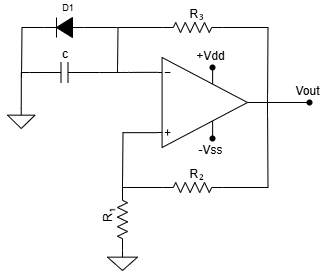
\includegraphics[width=0.5\linewidth]{immagini/monostabile/circuito_1.png}
	\caption{Una prima \textit{implementazione} del monostabile.}
	\label{fig:schematico_monostabile_1}
\end{figure}

Nella prima configurazione mostrata in figura \ref{fig:schematico_monostabile_1} con diodo collegato in parallelo alla capacità, il comportamento del circuito si può suddividere in due fasi: nella prima fase, la capacità si carica attraverso la resistenza fino a raggiungere circa \SI{0.7}{\volt}.
A questo punto il diodo entra in conduzione, offrendo un percorso a bassa resistenza alla corrente.
Di conseguenza, la carica del condensatore si arresta e l’uscita si stabilizza intorno a \SI{0.7}{\volt}.

\begin{figure}[h]
	\centering
	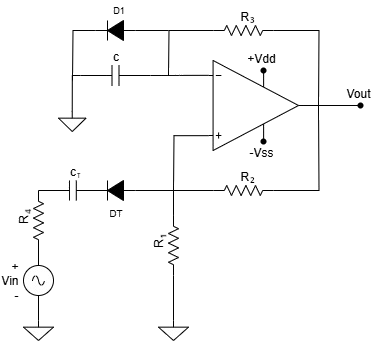
\includegraphics[width=0.6\linewidth]{immagini/monostabile/circuito.png}
	\caption{Schematico del circuito monostabile.}
	\label{fig:schematico_monostabile}
\end{figure}


L’aggiunta di un derivatore (filtro passa-alto) figura \ref{fig:schematico_monostabile}, consente di ottenere brevi impulsi in corrispondenza dei fronti del segnale di ingresso, modificando così il comportamento della soglia dinamica del circuito.
Collegando un diodo al derivatore si selezionano soltanto gli impulsi negativi, ottenendo un disaccoppiamento del segnale dal resto del circuito.

La durata dell'impulso $V_{out}$ è definita dalla costante $\tau$ e dalle resistenze $R_{1}$ e $R_{2}$:
\begin{align*}
	T_{A}=\tau\cdot\ln(1+\dfrac{R_{1}}{R_{2}}) \xrightarrow{R_1 = R_2 \,\text{e}\, \tau = 721\,\mu s } T_A = 499\,\mu s
\end{align*}

\noindent Nella tabella di seguito (tabella \ref{tab:monostabile}) sono presenti i valori dei componenti utilizzati nella realizzazione del circuito.
\begin{table}[h]
	\centering
	\setlength{\tabcolsep}{20pt}
	\begin{tabular}{c c | c c}
		\toprule
		\textbf{Grandezza} & \textbf{Valore}             & \textbf{Grandezza} & \textbf{Valore}            \\
		\midrule
		$freq$   & $100\,\mathrm{Hz}$ & $R_3$    & $10.3\,K\Omega$   \\
		$V_{DD}$ & $10\,V$            & $R_4$    & $9.0\,K\Omega$    \\
		$R_1$    & $9.0\,K\Omega$     & $C$      & $70\,\mathrm{nF}$ \\
		$R_2$    & $9.0\,K\Omega$     & $C_T$    & $1\,\mathrm{nF}$  \\
		\bottomrule
	\end{tabular}
	\caption{Valori utilizzati nel circuito monostabile.}
	\label{tab:monostabile}
\end{table}

% \begin{table}[h]
% 	\centering
% 	\setlength{\tabcolsep}{20pt}
% 	\begin{tabular}{c c}
% 		\toprule
% 		\textbf{Grandezza} & \textbf{Valore}             \\
% 		\midrule
% 		$freq$   & $100\,\mathrm{Hz}$ \\
% 		$V_{DD}$ & $10\,V$            \\
% 		$R_1$    & $9.0\,K\Omega$     \\
% 		$R_2$    & $9.0\,K\Omega$     \\
% 		$R_3$    & $10.3\,K\Omega$    \\
% 		$R_4$    & $9.0\,K\Omega$     \\
% 		$C$      & $70\,\mathrm{nF}$  \\
% 		$C_T$    & $1\,\mathrm{nF}$   \\
% 		\bottomrule
% 	\end{tabular}
% 	\caption{Valori utilizzati nel circuito monostabile.}
% 	\label{tab:monostabile}
% \end{table}

\noindent A figura \ref{fig:monostabile_impulso_durata} viene misurata la durata dell'impulso mentre a figura \ref{fig:monostabile_impulsi} viene mostrata una serie d'impulsi.
\begin{figure}[h]
	\centering
	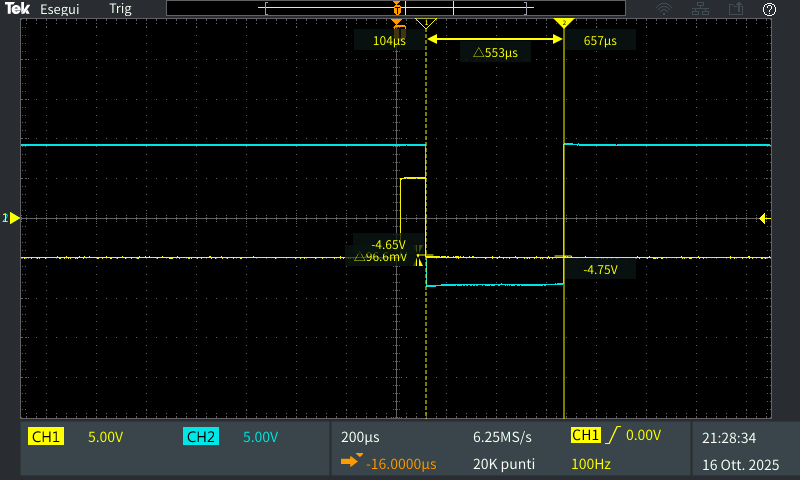
\includegraphics[width=0.7\linewidth]{immagini/monostabile/monostabile_durata.PNG}
	\caption{Impulso monostabile di durata $ 553\,\mu s$.}
	\label{fig:monostabile_impulso_durata}
\end{figure}

\begin{figure}[h]
	\centering
	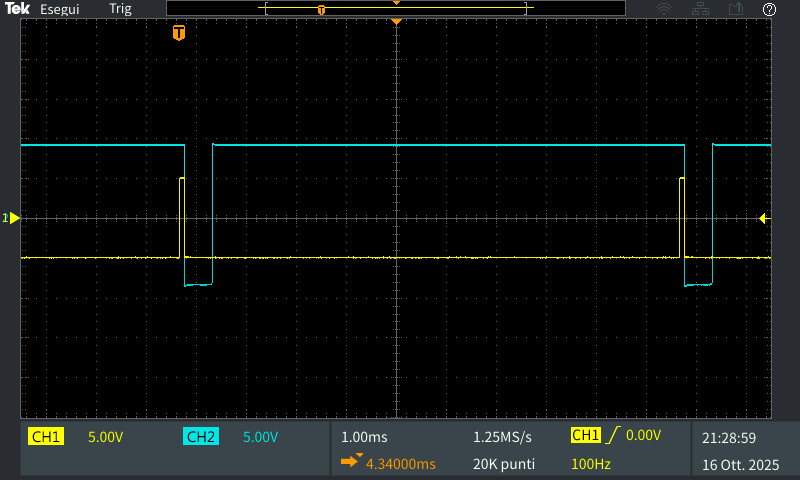
\includegraphics[width=0.7\linewidth]{immagini/monostabile/monostabile_impulsi.PNG}
	\caption{Serie d'impulsi del circuito monostabile.}
	\label{fig:monostabile_impulsi}
\end{figure}

\end{document}

